\documentclass[10pt,a4paper]{report}
\usepackage[utf8]{inputenc}
\usepackage[russian]{babel}
\usepackage[OT1]{fontenc}
\usepackage{amsmath}
\usepackage{amsfonts}
\usepackage{amssymb}
\usepackage{graphicx}
\author{Замотаева Юлия и Никитина Анна}
\title{Отчет по лабораторной работе по дисциплине: "Сети и системы передачи данных"\newline
тема: "Визуализация сигналов во временной и частотной области"}
\date{13.03.14}
\begin{document}
\maketitle
\pagebreak
\chapter{Теоретическая часть}
\section{Цель работы}
Познакомиться со средствами генерации сигналов и визуализации их спектров.
\section{Постановка задачи}
В командном окне MATLAB и в среде Simulink промоделировать чистый синусоидальный сигнал, так же синусоидальный сигнал с шумом. Получить их спектры.

\chapter{Ход работы}
\section{Код MATLAB для исходного сигнала}
x=0:0.01:4*pi;\newline
f0 = 20;\newline
\%исходный сигнал\newline
y = sin(2*pi*f0*x);\newline
figure(1)\newline
plot(x(1:200),y(1:200))\newline
grid\newline
\%спектр исходного сигнала\newline
figure(2)\newline
spectrum = fft(y,512);\newline
normspectrum = spectrum.*conj(spectrum)/512;\newline
f=100*(0:255)/512;\newline
plot(f, normspectrum(1:256))\newline
axis([0 max(F) 0 10])\newline
grid\newline

\section{Результаты работы программы}
В результате выполнения программы получились графики временной и частотной характеристик исходного синусоидальных сигнала. \newpage

\begin{figure}
\begin{center}
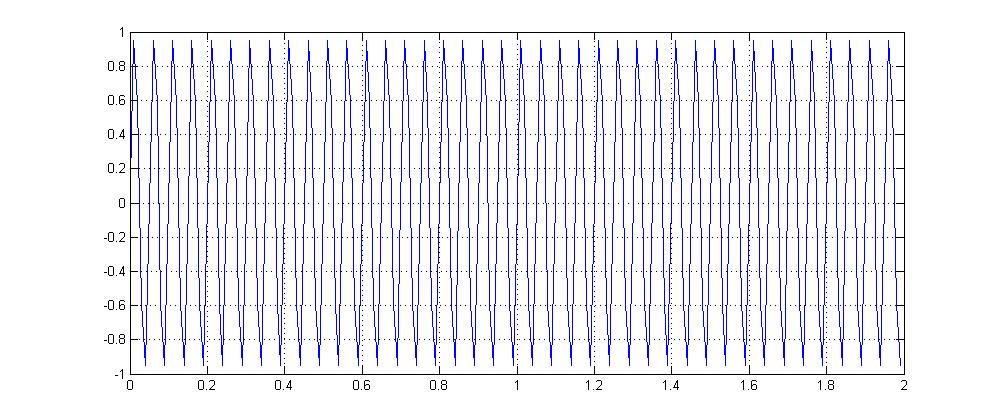
\includegraphics[angle=0, scale = 0.5]{1.png}\newline
рис. 1 Исходный сигнал\newline
\end{center}
\begin{center}
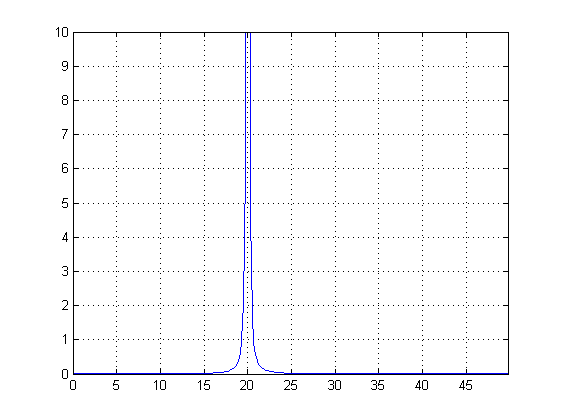
\includegraphics[angle=0, scale = 0.9]{2.png}\newline
рис. 2. Спектр исходного сигнала\newline
\end{center}
\end{figure}

\section{Код MATLAB для зашумленного сигнала}
\%зашумленный сигнал\newline
ynoize = y+ 0.5*rand(size(x));\newline
figure(3)\newline
plot(x(1:200),ynoize(1:200));\newline
grid\newline
\%спектр зашумленного сигнала\newline
spectrum = fft(ynoize,512);\newline
noizespectrum = spectrum.*conj(spectrum)/512;\newline
figure(4)\newline
plot(f, noizespectrum())\newline
axis([0 max(f) 0 10])\newline
grid\newline

\section{Результаты работы программы}
В результате выполнения программы получились графики временной и частотной характеристик зашумленного синусоидальных сигнала. \newpage

\begin{figure}
\begin{center}
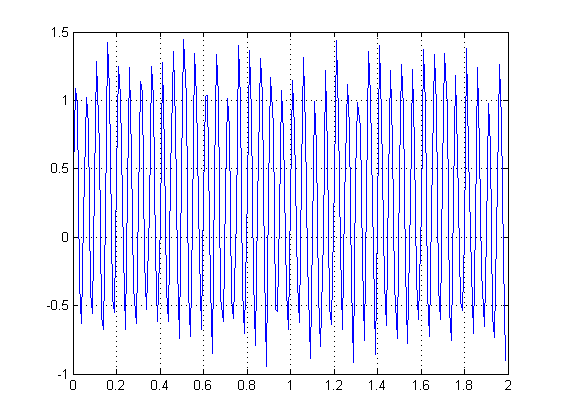
\includegraphics[angle=0, scale = 0.9]{3.png}\newline
рис. 3. Зашумленный сигнал\newline
\end{center}
\begin{center}
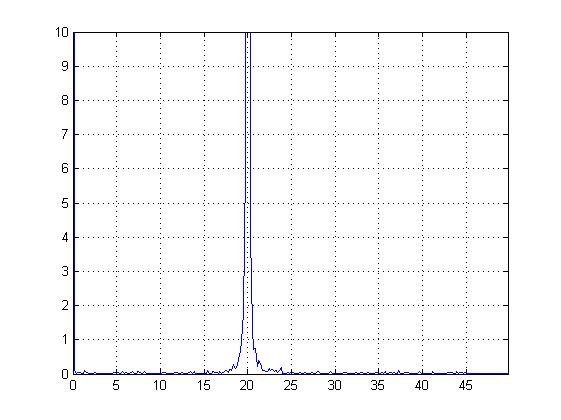
\includegraphics[angle=0, scale = 0.9]{4.png}\newline
рис. 4. Спектр зашумленного сигнала\newline
\end{center}
\end{figure}
\chapter{Вывод}
В данной работе мы построили исходный синусоидальный сигнал, после чего получили его спектр. Спектр представляет из себя резко возрастающий график. Далее построили зашумленный сигнал и его спектр. По рисункам видно, что они очень напонимают исходный сигнал, но являются более неровными.
\end{document}
